\chapter{Введение}\label{ch:introduction-ru}

Это руководство по эксплуатации охватывает цифровые приборные панели \ReplicaGenOne{} и \ReplicaNextLong{} для автомобилей Volkswagen Golf~II, Jetta~II и Scirocco~II.
В нём суммированы аппаратные версии, описаны их функции и приведены инструкции по установке, настройке, эксплуатации, хранению и обслуживанию приборов.
Рекомендации рассчитаны на владельцев автомобилей, автоэлектриков и сервисные центры, которые занимаются ретрофитом продукта.

В последующих главах приведены схема идентификации изделий, распиновка разъёмов, условия эксплуатации, а также подробные процедуры установки и конфигурации.
Дополнительно включены разделы по обслуживанию и диагностике обеих серий Replica, чтобы приборный щиток можно было обслуживать без заводской документации.

\begin{figure}[htbp]
    \centering
    \begin{subfigure}{0.48\textwidth}
        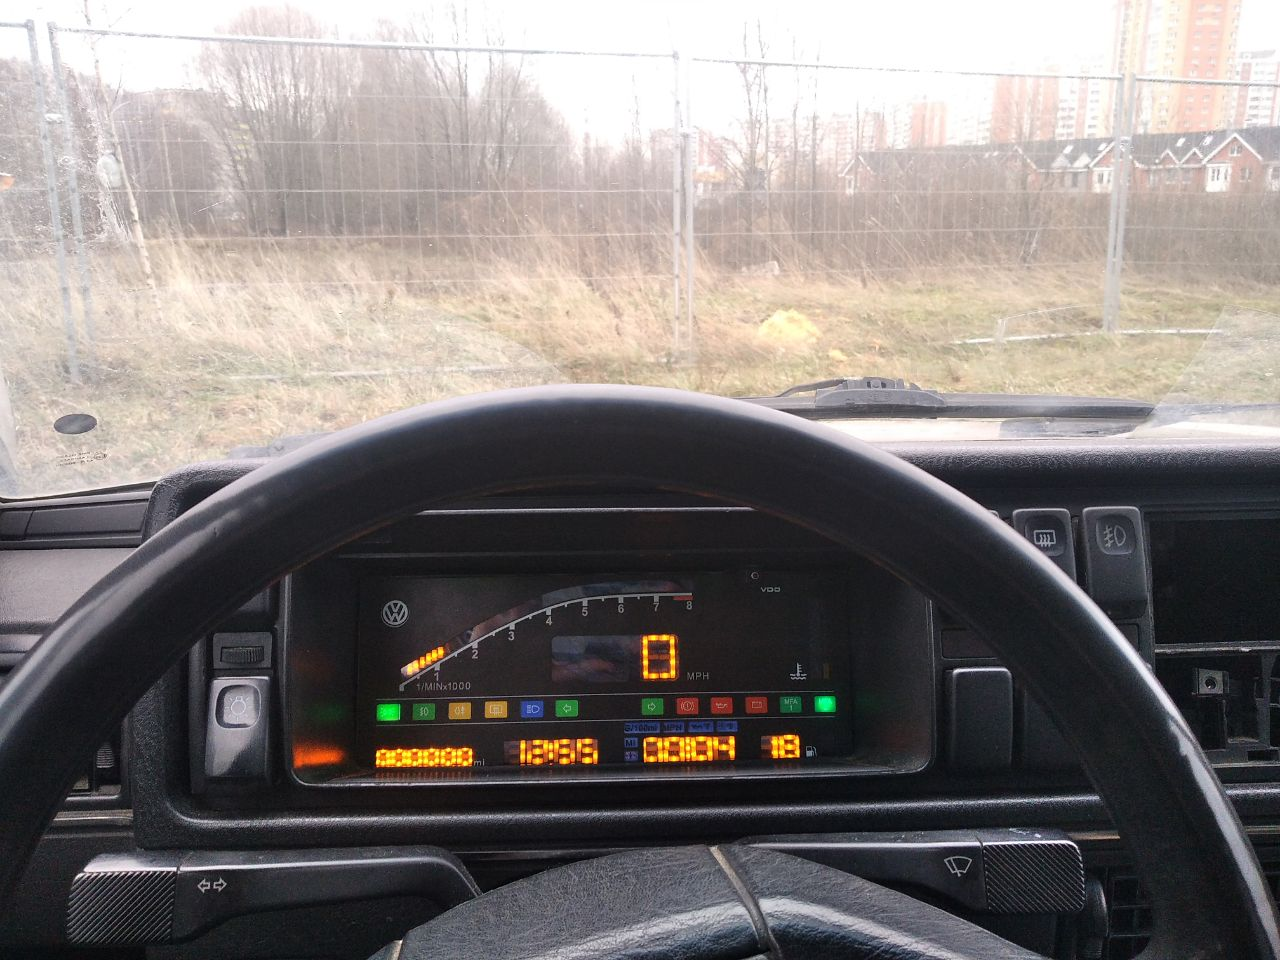
\includegraphics[width=\linewidth]{digifiz_manual/image004.jpg}
        \caption{Комплект поставки конфигурации GART~8--MGF.}
    \end{subfigure}\hfill
    \begin{subfigure}{0.48\textwidth}
        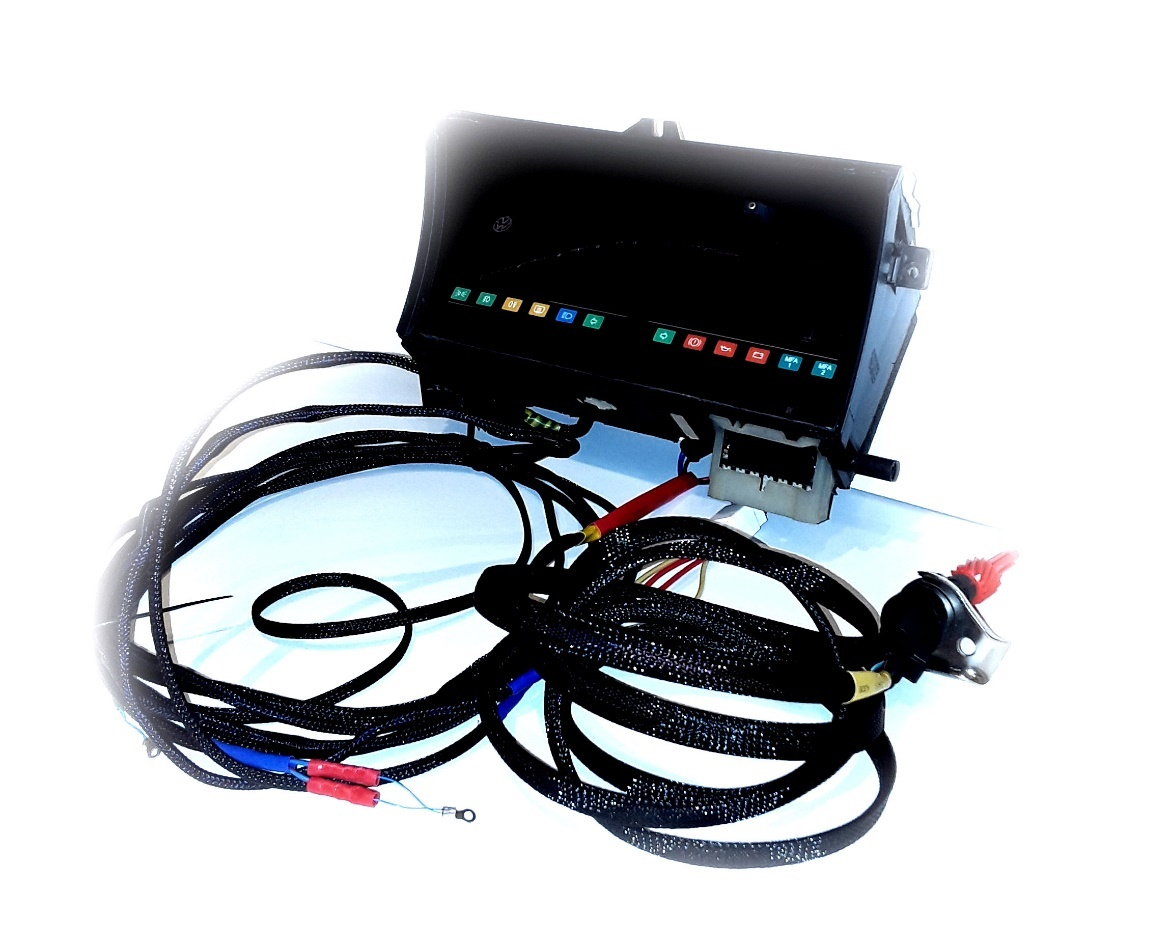
\includegraphics[width=\linewidth]{digifiz_manual/image005.jpg}
        \caption{Типичное содержимое комплекта GART.}
    \end{subfigure}
    \begin{subfigure}{0.48\textwidth}
        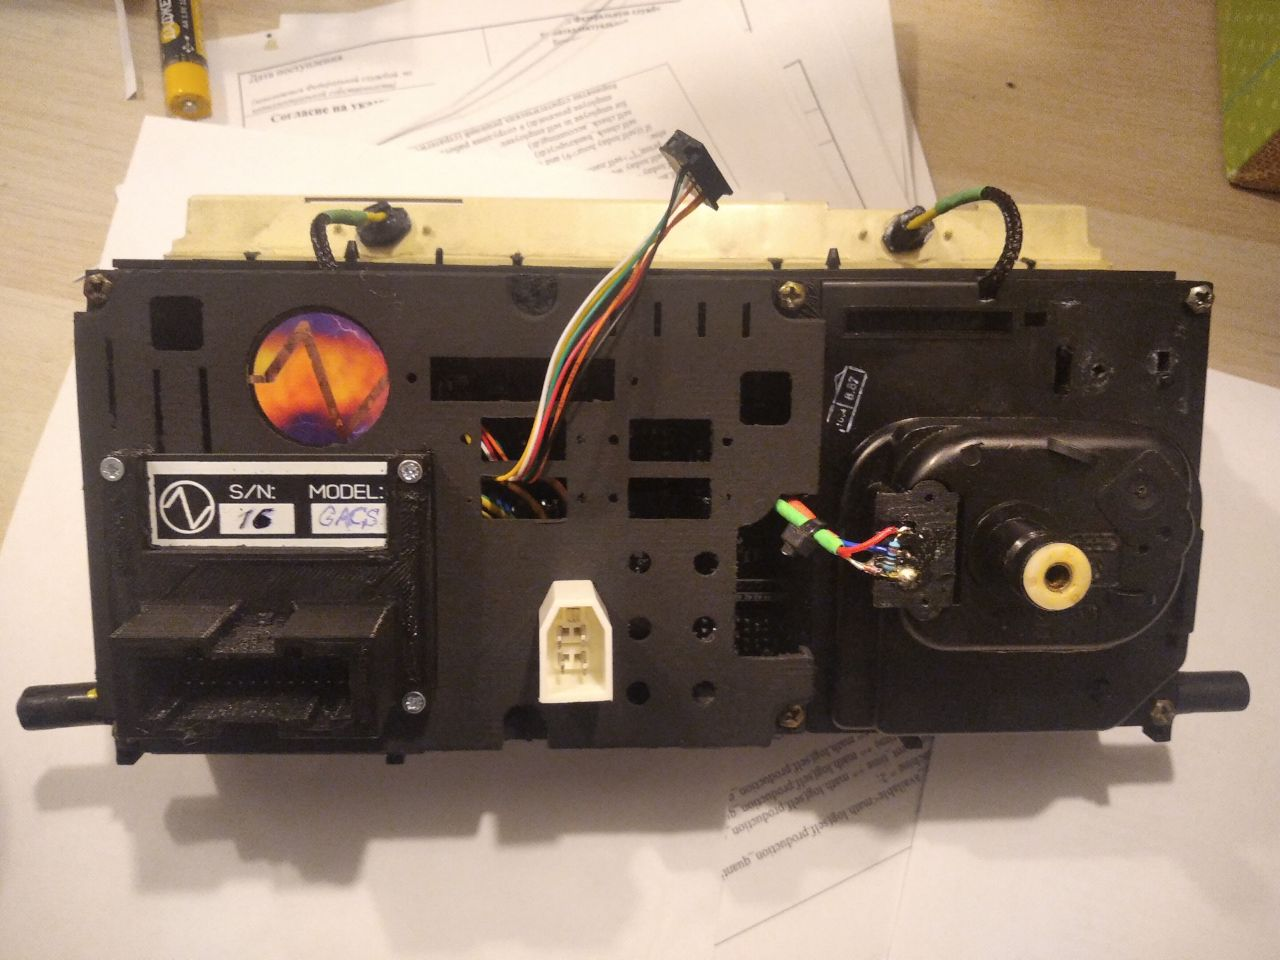
\includegraphics[width=\linewidth]{digifiz_manual/image006.jpg}
        \caption{Вид сзади на одноканальный модуль GACS.}
    \end{subfigure}\hfill
    \begin{subfigure}{0.48\textwidth}
        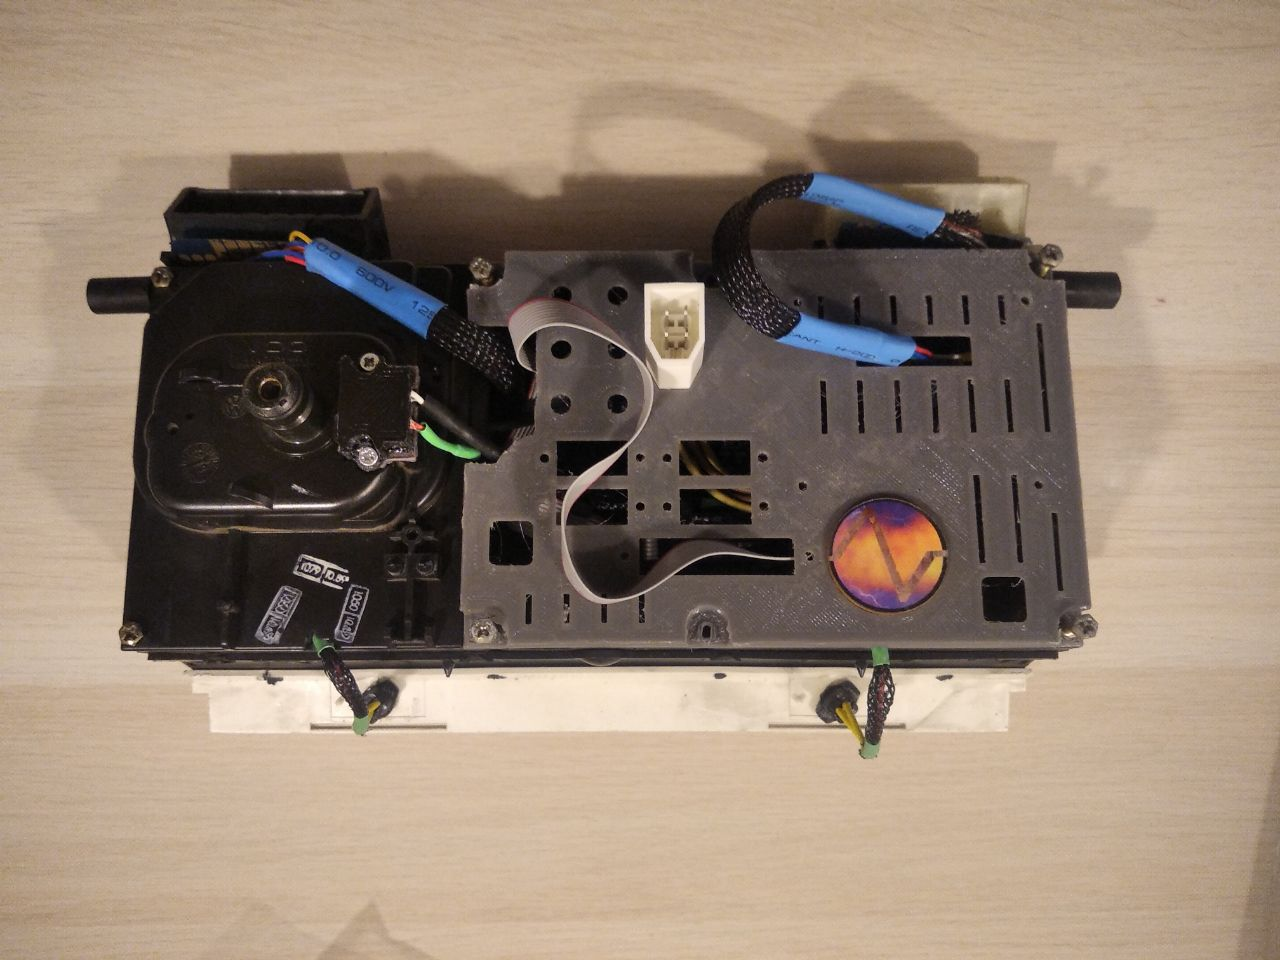
\includegraphics[width=\linewidth]{digifiz_manual/image007.jpg}
        \caption{Вид сзади на двухразъёмный модуль GACT.}
    \end{subfigure}
    \caption{Типовые приборные панели \ReplicaGenOne{} и \ReplicaNextLong{}, описанные в этом руководстве.}
\end{figure}

Каждая модификация поставляется с компонентами, необходимыми для соответствующего силового агрегата, единиц измерения и типа жгута.
В последующих главах расшифровываются обозначения модификаций и приводятся таблицы контактов, чтобы щиток можно было безопасно интегрировать.
